\begin{frame}{Benchmarks}
	\Large{\highlightB{Partitioning of the Snapshot matrix}}
	\normalsize

	\begin{minipage}[t]{0.3\textwidth}
		\scalebox{0.75}{
			\tikzset{
	main/.style={black, line width=0.4mm, opacity=1},
	second/.style={gray, opacity=5},
	arrow/.style={-latex, shorten >=1ex, shorten <=1ex, bend angle=45}
}
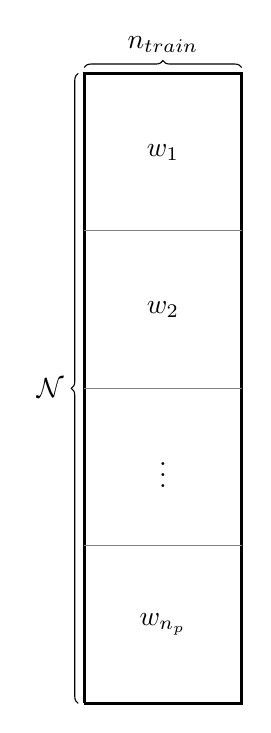
\begin{tikzpicture}
\draw[main] (0,0) -- (2,0) -- (2,8)-- (0,8)-- (0,0);

\draw[second] (0,2) -- (2,2) ;
\draw[second] (0,4) -- (2,4) ;
\draw[second] (0,6) -- (2,6) ;


\draw[decorate, decoration={brace,mirror}, yshift=.5ex]  (2,8) -- node[above=0.4ex] {$n_{train}$}  (0,8);
\draw[decorate, decoration={brace}, xshift=-.5ex]  (0,0) -- node[left=0.4ex] {$\mathcal{ N }$}  (0,8);

\draw (1,7) node {$w_1$};
\draw (1,5) node {$w_2$};
\draw (1,3) node {$\vdots$};
\draw (1,1) node {$w_{n_p}$};


\end{tikzpicture}
		}
	\end{minipage}
	\begin{minipage}[t]{0.6\textwidth}\vspace{-60mm}
		\begin{enumerate}
%			\item Scatter Snapshot matrix
			\item compute local correlation matrix $w_i^Tw_i$
			\item reduce local correlation matrices to get global correlation matrix $C$
			\item Solve EVP $C=V D V^T$
			\item compute $VD^{-\frac{1}{2}}$
			\item Broadcast $VD^{-\frac{1}{2}}$ to every processor
			\item $	u_i = w_i \cdot VD^{-\frac{1}{2}}$
%			\item Scatter POD vectors $u_i$ to $U$
		\end{enumerate}
	\end{minipage}
	
\end{frame}

%%%%%%%%%%%%%%%%%%%%%%%%%%%%%%%%%%%%%%%%%%%%%%%%%%%%%%%%%%%%%%%%%%%%%%%%%%%%%%%%
\begin{frame}{Benchmarks}
	\Large{\highlightB{Snapshot matrix is already distributed}}
	\normalsize random $10^7 \times 300 $ matrix
	
	\centering
	\scalebox{0.75}{
		% This file was created by matlab2tikz.
%
%The latest updates can be retrieved from
%  http://www.mathworks.com/matlabcentral/fileexchange/22022-matlab2tikz-matlab2tikz
%where you can also make suggestions and rate matlab2tikz.
%
\definecolor{mycolor1}{rgb}{0.00000,0.44700,0.74100}%
\definecolor{mycolor2}{rgb}{0.85000,0.32500,0.09800}%
\definecolor{mycolor3}{rgb}{0.92900,0.69400,0.12500}%
%
\begin{tikzpicture}

\begin{axis}[%
width=4.521in,
height=3.566in,
at={(0.758in,0.481in)},
scale only axis,
xmin=0,
xmax=82,
xlabel style={font=\color{white!15!black}},
xlabel={Number of Processors},
ymin=0,
ymax=82,
ylabel style={font=\color{white!15!black}},
ylabel={Speed up},
axis background/.style={fill=white},
axis x line*=bottom,
axis y line*=left,
legend style={at={(0.03,0.97)}, anchor=north west, legend cell align=left, align=left, draw=white!15!black}
]
\addplot [color=mycolor1]
  table[row sep=crcr]{%
1	1\\
2	2\\
3	3\\
4	4\\
5	5\\
6	6\\
7	7\\
8	8\\
9	9\\
10	10\\
11	11\\
12	12\\
13	13\\
14	14\\
15	15\\
16	16\\
17	17\\
18	18\\
19	19\\
20	20\\
21	21\\
22	22\\
23	23\\
24	24\\
25	25\\
26	26\\
27	27\\
28	28\\
29	29\\
30	30\\
31	31\\
32	32\\
33	33\\
34	34\\
35	35\\
36	36\\
37	37\\
38	38\\
39	39\\
40	40\\
41	41\\
42	42\\
43	43\\
44	44\\
45	45\\
46	46\\
47	47\\
48	48\\
49	49\\
50	50\\
51	51\\
52	52\\
53	53\\
54	54\\
55	55\\
56	56\\
57	57\\
58	58\\
59	59\\
60	60\\
61	61\\
62	62\\
63	63\\
64	64\\
65	65\\
66	66\\
67	67\\
68	68\\
69	69\\
70	70\\
71	71\\
72	72\\
73	73\\
74	74\\
75	75\\
76	76\\
77	77\\
78	78\\
79	79\\
80	80\\
};
\addlegendentry{optimum}

\addplot [color=mycolor2, mark=+, mark options={solid, mycolor2}]
  table[row sep=crcr]{%
1	1\\
2	1.90435312537314\\
3	2.91676067504077\\
4	3.86894083378637\\
5	4.67925489833916\\
6	5.60533428687974\\
7	6.31327396649857\\
8	7.18668106213769\\
9	7.8245179865632\\
10	8.64500211841435\\
11	9.18871604802155\\
12	9.9690296540242\\
13	10.7762433048319\\
14	11.4807987275723\\
15	12.2706171782628\\
16	13.0489929114543\\
17	13.6282138175286\\
18	14.5105890861279\\
19	15.1788657127022\\
20	15.8754357310119\\
21	16.6012961296239\\
22	17.5037604442592\\
23	18.2043788530567\\
24	18.956887827945\\
25	19.7576550541797\\
26	20.4713516836763\\
27	21.1570239669666\\
28	22.0555375224363\\
29	22.7011367116989\\
30	23.4438707674509\\
31	24.1966791048682\\
32	24.8578170131667\\
33	25.7765657561588\\
34	26.1958730121776\\
35	26.8408464997167\\
36	27.5378114624285\\
37	28.3248649789337\\
38	29.1315906905017\\
39	29.8626085928288\\
40	30.5755130400262\\
41	31.1078167173808\\
42	32.071334640588\\
43	32.4917517263081\\
44	33.7919461109117\\
45	33.250268091445\\
46	35.1360855502702\\
47	35.2971772530692\\
48	35.8046167802302\\
49	36.5996967419857\\
50	37.6756163149921\\
51	37.8542128158092\\
52	38.4860660946632\\
53	38.8758422518715\\
54	39.7383366342055\\
55	40.6289663333252\\
56	40.879341863036\\
57	41.6818090131215\\
58	42.242897953441\\
59	43.0484895789623\\
60	43.7119002245837\\
61	45.4525499804052\\
62	45.6409581743878\\
63	45.8895973423023\\
64	46.7448165168934\\
65	47.6476892263279\\
66	47.9609278664988\\
67	48.9572610052728\\
68	49.4263026876466\\
69	49.976566241854\\
70	50.6526351599004\\
71	50.5562512439251\\
72	51.1733682000738\\
73	52.0628534354749\\
74	52.310337961667\\
75	52.9005510589999\\
76	53.5381705285246\\
77	54.097982342764\\
78	55.1353374171769\\
79	54.9281112084495\\
80	56.0526199890084\\
};
\addlegendentry{EVP}

\addplot [color=mycolor3, mark=o, mark options={solid, mycolor3}]
  table[row sep=crcr]{%
1	1\\
2	1.89341734590023\\
3	3.18523814092857\\
4	4.04559628047612\\
5	4.93672404049657\\
6	5.8018981501777\\
7	6.28231202556641\\
8	7.11727245968104\\
9	7.44280518460258\\
10	8.19675963966155\\
11	8.30536662221775\\
12	8.81609508039606\\
13	8.99363921546519\\
14	9.85358150397242\\
15	9.45006714756788\\
16	10.0489412829876\\
17	10.4760604989543\\
18	10.5972082283826\\
19	10.477916778077\\
20	10.9054016343134\\
21	11.8055857953194\\
22	12.2712505850725\\
23	12.7240336347425\\
24	13.7398880653769\\
25	13.9045509048722\\
26	14.8503709245846\\
27	15.4864066111609\\
28	15.7628939093771\\
29	16.0854227775096\\
30	16.3538476945899\\
31	16.6431850365479\\
32	17.9468096366517\\
33	18.0845223536957\\
34	19.9267845776573\\
35	19.353337577975\\
36	20.656160455326\\
37	20.9832096141825\\
38	21.7511578958998\\
39	22.5719248994952\\
40	21.329374470285\\
41	22.5879698656227\\
42	22.7834540172868\\
43	23.9039954858414\\
44	25.2592478216008\\
45	24.1751067810007\\
46	26.41924965162\\
47	26.1152719448841\\
48	26.4943341958432\\
49	26.7597598120258\\
50	27.5482932472863\\
51	28.6274967374212\\
52	29.7174603700777\\
53	29.7672412988408\\
54	29.0743658599395\\
55	30.8626533854407\\
56	30.5672734817794\\
57	30.3053765473552\\
58	34.2409397021241\\
59	33.3798697603544\\
60	32.4570657306084\\
61	33.7168805553216\\
62	34.0967969578083\\
63	34.0496990535102\\
64	35.3767894689022\\
65	37.1955215369233\\
66	39.2665965428684\\
67	36.5812005693449\\
68	39.9099813123068\\
69	37.9187744506673\\
70	41.0608130633785\\
71	40.3214552369262\\
72	40.9744834357946\\
73	41.9863017351827\\
74	40.0864645458981\\
75	42.456231394801\\
76	42.6779028847483\\
77	41.988566713747\\
78	40.9513511131567\\
79	40.7350373128472\\
80	41.4621885686537\\
};
\addlegendentry{SVD}

\end{axis}
\end{tikzpicture}%
	}	
\end{frame}

%%%%%%%%%%%%%%%%%%%%%%%%%%%%%%%%%%%%%%%%%%%%%%%%%%%%%%%%%%%%%%%%%%%%%%%%%%%%%%%%
\begin{frame}{MPI}
	\Large{\highlightB{MPI\_Scatter}}
	\normalsize
	
	\centering
	\vspace{1cm}
	\tikzset{
	main/.style={black, line width=0.4mm, opacity=1},
	second/.style={gray, opacity=5},
	arrow/.style={-latex, shorten >=1ex, shorten <=1ex, bend angle=45}
}
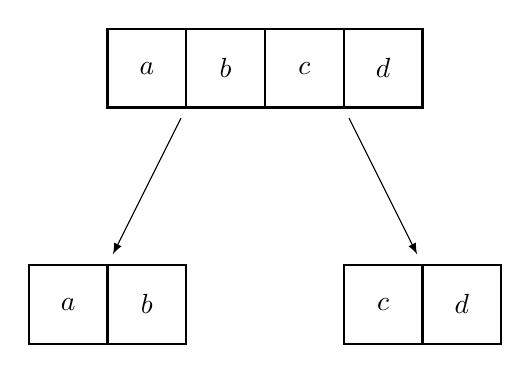
\begin{tikzpicture}
\node (rect) at (1,0) [draw,thick,minimum width=1cm,minimum height=1cm]  {$a$};
\node (rect) at (2,0) [draw,thick,minimum width=1cm,minimum height=1cm]  {$b$};
\node (rect) at (3,0) [draw,thick,minimum width=1cm,minimum height=1cm]  {$c$};
\node (rect) at (4,0) [draw,thick,minimum width=1cm,minimum height=1cm]  {$d$};

\node (rect) at (0,-3) [draw,thick,minimum width=1cm,minimum height=1cm] {$a$};
\node (rect) at (1,-3) [draw,thick,minimum width=1cm,minimum height=1cm] {$b$};

\node (rect) at (4,-3) [draw,thick,minimum width=1cm,minimum height=1cm] {$c$};
\node (rect) at (5,-3) [draw,thick,minimum width=1cm,minimum height=1cm] {$d$};


\draw [arrow]  (1.5,-0.5) to (0.5,-2.5);
\draw [arrow]  (3.5,-0.5) to (4.5,-2.5);

\end{tikzpicture}
	
\end{frame}

%%%%%%%%%%%%%%%%%%%%%%%%%%%%%%%%%%%%%%%%%%%%%%%%%%%%%%%%%%%%%%%%%%%%%%%%%%%%%%%%
\begin{frame}{MPI}
	\Large{\highlightB{MPI\_Gather}}
	\normalsize
	
	\centering
	\vspace{1cm}
	\tikzset{
	main/.style={black, line width=0.4mm, opacity=1},
	second/.style={gray, opacity=5},
	arrow/.style={-latex, shorten >=1ex, shorten <=1ex, bend angle=45}
}
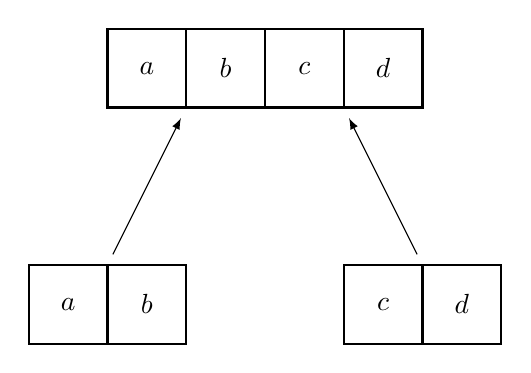
\begin{tikzpicture}
\node (rect) at (1,0) [draw,thick,minimum width=1cm,minimum height=1cm]  {$a$};
\node (rect) at (2,0) [draw,thick,minimum width=1cm,minimum height=1cm]  {$b$};
\node (rect) at (3,0) [draw,thick,minimum width=1cm,minimum height=1cm]  {$c$};
\node (rect) at (4,0) [draw,thick,minimum width=1cm,minimum height=1cm]  {$d$};

\node (rect) at (0,-3) [draw,thick,minimum width=1cm,minimum height=1cm] {$a$};
\node (rect) at (1,-3) [draw,thick,minimum width=1cm,minimum height=1cm] {$b$};

\node (rect) at (4,-3) [draw,thick,minimum width=1cm,minimum height=1cm] {$c$};
\node (rect) at (5,-3) [draw,thick,minimum width=1cm,minimum height=1cm] {$d$};


\draw [arrow]  (0.5,-2.5) to (1.5,-0.5) ;
\draw [arrow]  (4.5,-2.5) to (3.5,-0.5) ;

\end{tikzpicture}
	
\end{frame}

%%%%%%%%%%%%%%%%%%%%%%%%%%%%%%%%%%%%%%%%%%%%%%%%%%%%%%%%%%%%%%%%%%%%%%%%%%%%%%%%
\begin{frame}{MPI}
	\Large{\highlightB{MPI\_Scatterv and MPI\_Gatherv}}
	\normalsize
	
	\vspace{1cm}
	\centering\tikzset{
	main/.style={black, line width=0.4mm, opacity=1},
	second/.style={gray, opacity=5},
	arrow/.style={-latex, shorten >=1ex, shorten <=1ex, bend angle=45}
}
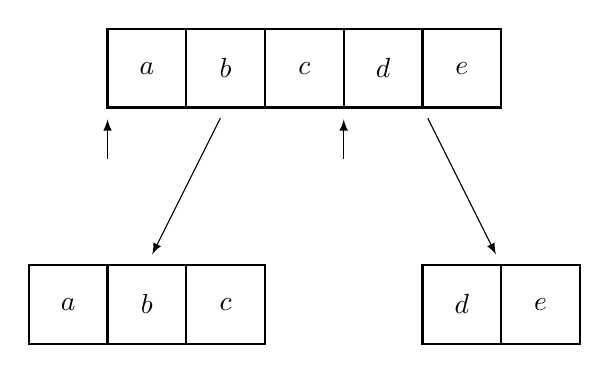
\begin{tikzpicture}
\node (rect) at (1,0) [draw,thick,minimum width=1cm,minimum height=1cm]  {$a$};
\node (rect) at (2,0) [draw,thick,minimum width=1cm,minimum height=1cm]  {$b$};
\node (rect) at (3,0) [draw,thick,minimum width=1cm,minimum height=1cm]  {$c$};
\node (rect) at (4,0) [draw,thick,minimum width=1cm,minimum height=1cm]  {$d$};
\node (rect) at (5,0) [draw,thick,minimum width=1cm,minimum height=1cm]  {$e$};

\node (rect) at (0,-3) [draw,thick,minimum width=1cm,minimum height=1cm] {$a$};
\node (rect) at (1,-3) [draw,thick,minimum width=1cm,minimum height=1cm] {$b$};
\node (rect) at (2,-3) [draw,thick,minimum width=1cm,minimum height=1cm] {$c$};

\node (rect) at (5,-3) [draw,thick,minimum width=1cm,minimum height=1cm] {$d$};
\node (rect) at (6,-3) [draw,thick,minimum width=1cm,minimum height=1cm] {$e$};


\draw [arrow]  (2,-0.5) to (1,-2.5);
\draw [arrow]  (4.5,-0.5) to (5.5,-2.5);

\draw [arrow]  (.5, -1.3) to (.5, -0.5);
\draw [arrow]  (3.5, -1.3) to (3.5, -0.5);
\end{tikzpicture}	
	
	\vspace{1cm}
	sendcount = [3,2], displacement = [0,3]
\end{frame}

%%%%%%%%%%%%%%%%%%%%%%%%%%%%%%%%%%%%%%%%%%%%%%%%%%%%%%%%%%%%%%%%%%%%%%%%%%%%%%%%
\begin{frame}{Benchmarks}
	\Large{\highlightB{With scattering and gathering of $\mathcal{ W }$}}
	\normalsize  random $10^7 \times 300 $ matrix
	
	\centering
	\scalebox{0.75}{
		% This file was created by matlab2tikz.
%
%The latest updates can be retrieved from
%  http://www.mathworks.com/matlabcentral/fileexchange/22022-matlab2tikz-matlab2tikz
%where you can also make suggestions and rate matlab2tikz.
%
\definecolor{mycolor1}{rgb}{0.00000,0.44700,0.74100}%
\definecolor{mycolor2}{rgb}{0.85000,0.32500,0.09800}%
\definecolor{mycolor3}{rgb}{0.92900,0.69400,0.12500}%
%
\begin{tikzpicture}

\begin{axis}[%
width=4.521in,
height=3.566in,
at={(0.758in,0.481in)},
scale only axis,
xmin=0,
xmax=82,
xlabel style={font=\color{white!15!black}},
xlabel={Number of Processors},
ymin=0,
ymax=82,
ylabel style={font=\color{white!15!black}},
ylabel={Speed up},
axis background/.style={fill=white},
axis x line*=bottom,
axis y line*=left,
legend style={at={(0.03,0.97)}, anchor=north west, legend cell align=left, align=left, draw=white!15!black}
]
\addplot [color=mycolor1]
  table[row sep=crcr]{%
1	1\\
2	2\\
3	3\\
4	4\\
5	5\\
6	6\\
7	7\\
8	8\\
9	9\\
10	10\\
11	11\\
12	12\\
13	13\\
14	14\\
15	15\\
16	16\\
17	17\\
18	18\\
19	19\\
20	20\\
21	21\\
22	22\\
23	23\\
24	24\\
25	25\\
26	26\\
27	27\\
28	28\\
29	29\\
30	30\\
31	31\\
32	32\\
33	33\\
34	34\\
35	35\\
36	36\\
37	37\\
38	38\\
39	39\\
40	40\\
41	41\\
42	42\\
43	43\\
44	44\\
45	45\\
46	46\\
47	47\\
48	48\\
49	49\\
50	50\\
51	51\\
52	52\\
53	53\\
54	54\\
55	55\\
56	56\\
57	57\\
58	58\\
59	59\\
60	60\\
61	61\\
62	62\\
63	63\\
64	64\\
65	65\\
66	66\\
67	67\\
68	68\\
69	69\\
70	70\\
71	71\\
72	72\\
73	73\\
74	74\\
75	75\\
76	76\\
77	77\\
78	78\\
79	79\\
80	80\\
};
\addlegendentry{optimum}

\addplot [color=mycolor2, mark=x, mark options={solid, mycolor2}]
  table[row sep=crcr]{%
1	1\\
2	1.77735939387169\\
3	2.52863802350192\\
4	3.11057452110864\\
5	3.57893371259742\\
6	4.03232957353491\\
7	4.36130918935323\\
8	4.67456634083019\\
9	4.96249680943954\\
10	5.18947108447311\\
11	5.3335858729696\\
12	5.57220230405285\\
13	5.77127895622898\\
14	5.93399104352579\\
15	6.12791655430983\\
16	6.28131741232361\\
17	6.43572939044164\\
18	6.56942710425942\\
19	6.66259136120854\\
20	6.80310003314158\\
21	6.8629704671702\\
22	6.95050381730676\\
23	7.0026864165578\\
24	6.92879415004413\\
25	7.08846366609532\\
26	6.9958134809417\\
27	7.1537590661212\\
28	7.24624355476011\\
29	7.25119069143157\\
30	7.31806814919965\\
31	7.22171902050757\\
32	7.36785127600237\\
33	7.44764432815705\\
34	7.34539780745157\\
35	7.47319736513956\\
36	7.39081520555148\\
37	7.36910800431576\\
38	7.38777309107804\\
39	7.3566343535053\\
40	7.36808456825069\\
41	7.3834996696319\\
42	7.40378336312328\\
43	7.456569802935\\
44	7.05333438969816\\
45	7.43337465868924\\
46	7.50542861816718\\
47	7.43100346348961\\
48	7.42223143860942\\
49	7.52852347272102\\
50	7.53526729861858\\
51	7.46282625617122\\
52	7.5158741513344\\
53	7.43827655521545\\
54	7.33350964058771\\
55	7.52955433241322\\
56	7.39065330756398\\
57	7.4887936570745\\
58	7.45271351948498\\
59	7.52831060218862\\
60	7.4980138562886\\
61	7.55635737800393\\
62	7.50499860940941\\
63	7.29286168282935\\
64	7.37136455145628\\
65	7.63115952606785\\
66	7.64077429773524\\
67	7.56358721651871\\
68	7.52144777572109\\
69	7.62030948823592\\
70	7.56761881561985\\
71	7.54313696293749\\
72	7.54849495681635\\
73	7.64542909527055\\
74	7.52888257463664\\
75	7.49192020751487\\
76	7.61477515161743\\
77	7.57164503375542\\
78	7.23160517512624\\
79	7.56567980540322\\
80	7.43390429934376\\
};
\addlegendentry{EVP}

\addplot [color=mycolor3, mark=+, mark options={solid, mycolor3}]
  table[row sep=crcr]{%
1	0.0644134706630309\\
2	0.121429810853809\\
3	0.203059284116331\\
4	0.256646008309173\\
5	0.311793484970624\\
6	0.364439924281973\\
7	0.393574070678828\\
8	0.443575708891036\\
9	0.462701461130375\\
10	0.506551521730153\\
11	0.512516891690243\\
12	0.541871584354609\\
13	0.551957233723199\\
14	0.600377954132289\\
15	0.576915306393257\\
16	0.609928612272296\\
17	0.633478092469771\\
18	0.639390998075112\\
19	0.632072161267883\\
20	0.653903688134457\\
21	0.703010508389928\\
22	0.727595190380761\\
23	0.751763534247655\\
24	0.805199339831863\\
25	0.815845004180602\\
26	0.86419572360972\\
27	0.894410122600335\\
28	0.908731664726426\\
29	0.925555040556199\\
30	0.939715730318634\\
31	0.954852378622423\\
32	1.01768985522706\\
33	1.02325037240064\\
34	1.11335064312017\\
35	1.08006937063289\\
36	1.14745102362626\\
37	1.15847348893686\\
38	1.19284917481663\\
39	1.22663164360764\\
40	1.16670591192576\\
41	1.22460234606197\\
42	1.23698676808494\\
43	1.27660035830304\\
44	1.34026449080253\\
45	1.29625770853619\\
46	1.39253918571556\\
47	1.38203854820538\\
48	1.40149434855347\\
49	1.40707510917746\\
50	1.44135858526514\\
51	1.48392878128024\\
52	1.53295285957849\\
53	1.53949413272853\\
54	1.49700663371601\\
55	1.56982074298877\\
56	1.57334435781624\\
57	1.54259173426033\\
58	1.71468049204225\\
59	1.66987981447088\\
60	1.63021852424936\\
61	1.68323557951482\\
62	1.6929761036298\\
63	1.68244403515131\\
64	1.73870543818423\\
65	1.8079538252603\\
66	1.88368433291433\\
67	1.78779788023682\\
68	1.90699247894872\\
69	1.83737322943827\\
70	1.94502520018575\\
71	1.91445438218831\\
72	1.94926845159181\\
73	1.96340438910897\\
74	1.90960707478878\\
75	1.97623336137365\\
76	1.99080609673254\\
77	1.97157999995408\\
78	1.92223091560331\\
79	1.91312355665274\\
80	1.94258302791729\\
};
\addlegendentry{SVD}

\end{axis}
\end{tikzpicture}%
	}	
\end{frame}

%%%%%%%%%%%%%%%%%%%%%%%%%%%%%%%%%%%%%%%%%%%%%%%%%%%%%%%%%%%%%%%%%%%%%%%%%%%%%%%%
\begin{frame}{nonblocking communication}
	\Large{\highlightB{MPI} \highlight{I} \highlightB{functions}}
	
	\begin{itemize}
		\item \highlight{I} functions provide non bocking communication
		\item communication is not blocking processor
		\item communication buffer should not be used while communication	
		\item MPI\_Scatterv $\Rightarrow$ MPI\_\highlight{I}scatterv  
		\item MPI\_Gatherv $\Rightarrow$ MPI\_\highlight{I}gatherv

	\end{itemize}	
\end{frame}

%%%%%%%%%%%%%%%%%%%%%%%%%%%%%%%%%%%%%%%%%%%%%%%%%%%%%%%%%%%%%%%%%%%%%%%%%%%%%%%%
\begin{frame}{nonblocking communication}
	\Large{\highlightB{Partitioning for non-blocking communication}}
	\normalsize
	
	\centering
	\scalebox{0.75}{
		\tikzset{
	main/.style={black, line width=0.4mm, opacity=1},
	second/.style={gray, opacity=5},
	arrow/.style={-latex, shorten >=1ex, shorten <=1ex, bend angle=45}
}
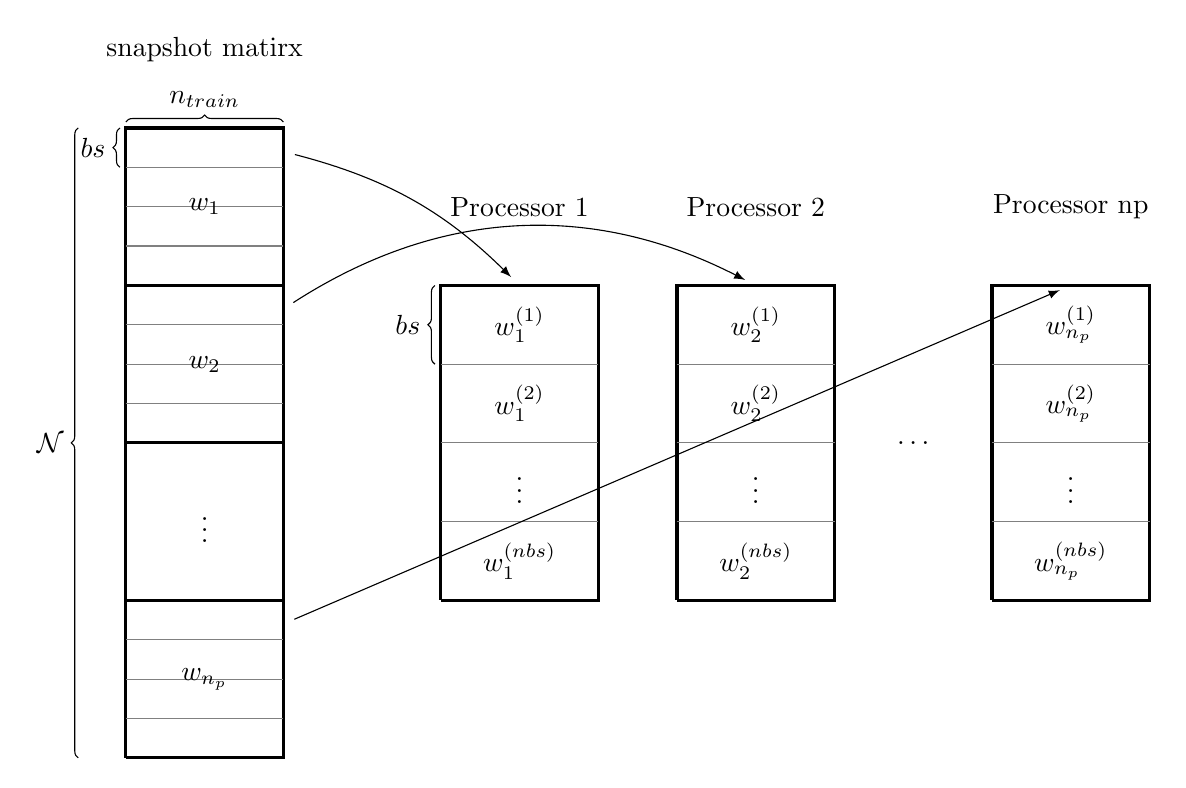
\begin{tikzpicture}
%% Snapshot Matrix
\draw (1,9) node {snapshot matirx};
\draw[main] (0,0) -- (2,0) -- (2,8)-- (0,8)-- (0,0);
\draw[main] (0,2) -- (2,2) ;
\draw[main] (0,4) -- (2,4) ;
\draw[main] (0,6) -- (2,6) ;

\draw[second] (0,7.5) -- (2,7.5) ;
\draw[second] (0,7) -- (2,7) ;
\draw[second] (0,6.5) -- (2,6.5) ;

\draw[second] (0,5.5) -- (2,5.5) ;
\draw[second] (0,5) -- (2,5) ;
\draw[second] (0,4.5) -- (2,4.5) ;

\draw[second] (0,1.5) -- (2,1.5) ;
\draw[second] (0,1) -- (2,1) ;
\draw[second] (0,.5) -- (2,.5) ;

\draw[decorate, decoration={brace,mirror}, yshift=.5ex]  (2,8) -- node[above=0.4ex] {$n_{train}$}  (0,8);
\draw[decorate, decoration={brace}, xshift=-4ex]  (0,0) -- node[left=0.4ex] {$\mathcal{ N }$}  (0,8);
\draw[decorate, decoration={brace}, xshift=-.5ex]  (0,7.5) -- node[left=0.4ex] {$bs$}  (0,8);

\draw (1,7) node {$w_1$};
\draw (1,5) node {$w_2$};
\draw (1,3) node {$\vdots$};
\draw (1,1) node {$w_{n_p}$};

%% prozessor1 Matrix
\draw (5,7) node {Processor 1};
\draw[main] (4,2) -- (6,2) -- (6,6)-- (4,6)-- (4,2);
\draw[second] (4,3) -- (6,3) ;
\draw[second] (4,4) -- (6,4) ;
\draw[second] (4,5) -- (6,5) ;

\draw (5,5.5) node {$w_1^{(1)}$};
\draw (5,4.5) node {$w_1^{(2)}$};
\draw (5,3.5) node {$\vdots$};
\draw (5,2.5) node {$w_{1}^{(nbs)}$};

\draw[decorate, decoration={brace}, xshift=-.5ex]  (4,5) -- node[left=0.4ex] {$bs$}  (4,6);

%% prozessor2 Matrix
\draw (8,7) node {Processor 2};
\draw[main] (7,2) -- (9,2) -- (9,6)-- (7,6)-- (7,2);
\draw[second] (7,3) -- (9,3) ;
\draw[second] (7,4) -- (9,4) ;
\draw[second] (7,5) -- (9,5) ;

\draw (8,5.5) node {$w_2^{(1)}$};
\draw (8,4.5) node {$w_2^{(2)}$};
\draw (8,3.5) node {$\vdots$};
\draw (8,2.5) node {$w_{2}^{(nbs)}$};

%% Dots
\draw (10,4) node {$\dots$};

%% prozessor np Matrix
\draw (12,7) node {Processor np};
\draw[main] (11,2) -- (13,2) -- (13,6)-- (11,6)-- (11,2);
\draw[gray] (11,3) -- (13,3) ;
\draw[gray] (11,4) -- (13,4) ;
\draw[gray] (11,5) -- (13,5) ;

\draw (12,5.5) node {$w_{n_p}^{(1)}$};
\draw (12,4.5) node {$w_{n_p}^{(2)}$};
\draw (12,3.5) node {$\vdots$};
\draw (12,2.5) node {$w_{n_p}^{(nbs)}$};

%% Pfeile
\draw [arrow, bend angle=15, bend left]  (2,7.7) to (5,6);
\draw [arrow, bend angle=30, bend left]  (2,5.7) to (8,6);

\draw [arrow, ]  (2,1.7) to (12,6);


\end{tikzpicture}
	}	
\end{frame}

%%%%%%%%%%%%%%%%%%%%%%%%%%%%%%%%%%%%%%%%%%%%%%%%%%%%%%%%%%%%%%%%%%%%%%%%%%%%%%%%
\begin{frame}{Benchmarks}
	\Large{\highlightB{Different block sizes}}
	\normalsize  random $10^7 \times 300 $ matrix
	
	\centering
	\scalebox{0.75}{
		% This file was created by matlab2tikz.
%
%The latest updates can be retrieved from
%  http://www.mathworks.com/matlabcentral/fileexchange/22022-matlab2tikz-matlab2tikz
%where you can also make suggestions and rate matlab2tikz.
%
\definecolor{mycolor1}{rgb}{0.00000,0.44700,0.74100}%
\definecolor{mycolor2}{rgb}{0.85000,0.32500,0.09800}%
\definecolor{mycolor3}{rgb}{0.92900,0.69400,0.12500}%
\definecolor{mycolor4}{rgb}{0.49400,0.18400,0.55600}%
\definecolor{mycolor5}{rgb}{0.46600,0.67400,0.18800}%
\definecolor{mycolor6}{rgb}{0.30100,0.74500,0.93300}%
\definecolor{mycolor7}{rgb}{0.63500,0.07800,0.18400}%
%
\begin{tikzpicture}

\begin{axis}[%
width=4.521in,
height=3.566in,
at={(0.758in,0.481in)},
scale only axis,
xmin=0,
xmax=82,
xlabel style={font=\color{white!15!black}},
xlabel={Number of Processors},
ymin=0,
ymax=8.2,
ylabel style={font=\color{white!15!black}},
ylabel={Speed up},
axis background/.style={fill=white},
axis x line*=bottom,
axis y line*=left,
legend style={at={(0.97,0.03)}, anchor=south east, legend cell align=left, align=left, draw=white!15!black}
]
\addplot [color=mycolor1]
  table[row sep=crcr]{%
1	1\\
2	1.77735939387169\\
3	2.52863802350192\\
4	3.11057452110864\\
5	3.57893371259742\\
6	4.03232957353491\\
7	4.36130918935323\\
8	4.67456634083019\\
9	4.96249680943954\\
10	5.18947108447311\\
11	5.3335858729696\\
12	5.57220230405285\\
13	5.77127895622898\\
14	5.93399104352579\\
15	6.12791655430983\\
16	6.28131741232361\\
17	6.43572939044164\\
18	6.56942710425942\\
19	6.66259136120854\\
20	6.80310003314158\\
21	6.8629704671702\\
22	6.95050381730676\\
23	7.0026864165578\\
24	6.92879415004413\\
25	7.08846366609532\\
26	6.9958134809417\\
27	7.1537590661212\\
28	7.24624355476011\\
29	7.25119069143157\\
30	7.31806814919965\\
31	7.22171902050757\\
32	7.36785127600237\\
33	7.44764432815705\\
34	7.34539780745157\\
35	7.47319736513956\\
36	7.39081520555148\\
37	7.36910800431576\\
38	7.38777309107804\\
39	7.3566343535053\\
40	7.36808456825069\\
41	7.3834996696319\\
42	7.40378336312328\\
43	7.456569802935\\
44	7.05333438969816\\
45	7.43337465868924\\
46	7.50542861816718\\
47	7.43100346348961\\
48	7.42223143860942\\
49	7.52852347272102\\
50	7.53526729861858\\
51	7.46282625617122\\
52	7.5158741513344\\
53	7.43827655521545\\
54	7.33350964058771\\
55	7.52955433241322\\
56	7.39065330756398\\
57	7.4887936570745\\
58	7.45271351948498\\
59	7.52831060218862\\
60	7.4980138562886\\
61	7.55635737800393\\
62	7.50499860940941\\
63	7.29286168282935\\
64	7.37136455145628\\
65	7.63115952606785\\
66	7.64077429773524\\
67	7.56358721651871\\
68	7.52144777572109\\
69	7.62030948823592\\
70	7.56761881561985\\
71	7.54313696293749\\
72	7.54849495681635\\
73	7.64542909527055\\
74	7.52888257463664\\
75	7.49192020751487\\
76	7.61477515161743\\
77	7.57164503375542\\
78	7.23160517512624\\
79	7.56567980540322\\
80	7.43390429934376\\
};
\addlegendentry{unblocked}

\addplot [color=mycolor2]
  table[row sep=crcr]{%
1	0.560104987818282\\
2	0.838588924101627\\
3	1.19594770012883\\
4	1.60629405492368\\
5	2.17418195399243\\
6	2.44700259045947\\
7	2.68477826189594\\
8	2.97611769843718\\
9	3.13515352442571\\
10	3.39337200961901\\
11	3.54254821874291\\
12	3.63327324849523\\
13	3.78769307116311\\
14	4.0243550987505\\
15	4.187423740716\\
16	4.28513955913984\\
17	4.43369572513645\\
18	4.49600514181891\\
19	4.48782763901302\\
20	4.60293036856762\\
21	4.24008962520369\\
22	4.666481256046\\
23	4.66147793065821\\
24	4.35734482557387\\
25	4.50136719517917\\
26	4.73436834052407\\
27	4.76442056668525\\
28	4.67401277560496\\
29	4.67747550708572\\
30	4.74632788036073\\
31	4.71752630277724\\
32	4.74724631030737\\
33	4.75280382367267\\
34	4.72764314482273\\
35	4.36672930323388\\
36	4.70339145057569\\
37	4.79109781274411\\
38	4.77172814293058\\
39	4.80122426499368\\
40	4.76461884627336\\
41	4.90559453144192\\
42	4.82747491840928\\
43	4.71265868289765\\
44	4.91251269376768\\
45	5.02255221951205\\
46	4.78179942473207\\
47	4.9557502791958\\
48	5.12472538458095\\
49	5.11677015487477\\
50	5.20687500378997\\
51	5.33860078338722\\
52	5.22375863873071\\
53	5.21169453102002\\
54	5.26040121055437\\
55	5.61733721926743\\
56	5.32520830167851\\
57	5.21468553764682\\
58	5.35685218226736\\
59	5.43220534135517\\
60	5.47355083203452\\
61	5.52092092446079\\
62	5.80140768466782\\
63	5.49565613929539\\
64	5.84357361117727\\
65	5.83930165897646\\
66	5.61820094153518\\
67	5.36958170743909\\
68	5.99413996509599\\
69	5.57644207039875\\
70	5.62902914944458\\
71	6.13817826340264\\
72	5.85478983632155\\
73	5.65641357548929\\
74	5.62083049671388\\
75	5.55344996523679\\
76	5.84986374443907\\
77	5.75824294101671\\
78	5.87319117647059\\
79	5.54044250728317\\
80	5.65635768373138\\
};
\addlegendentry{BS40}

\addplot [color=mycolor3]
  table[row sep=crcr]{%
1	0.702671082942238\\
2	0.886661314305776\\
3	1.25132694549694\\
4	1.65931156759682\\
5	2.05489762731821\\
6	2.46598396907542\\
7	2.72630463496257\\
8	3.11235757328621\\
9	3.26129151102308\\
10	3.5101239044411\\
11	3.58187891466627\\
12	3.72811978985759\\
13	3.90968450624704\\
14	4.11134490295736\\
15	4.24462748432352\\
16	4.43907073526941\\
17	4.56849762572991\\
18	4.42432926106648\\
19	4.57049164184904\\
20	4.67691501153351\\
21	5.10551333963599\\
22	5.29599312914009\\
23	5.52600178266312\\
24	5.638214166114\\
25	5.8621445224628\\
26	5.89346760743186\\
27	5.98292589457108\\
28	5.95570333172648\\
29	6.02332101069054\\
30	5.99566765702954\\
31	6.27038717969315\\
32	6.14426153846154\\
33	6.19835018281173\\
34	6.26464584192114\\
35	6.24909883519946\\
36	6.28208532088613\\
37	6.29495764435924\\
38	6.35165030661232\\
39	6.51789181639454\\
40	6.22150164837155\\
41	6.49052341556149\\
42	6.58595654925121\\
43	6.52044081632653\\
44	6.44250696838622\\
45	6.7269686512149\\
46	6.76305040425004\\
47	6.755574568857\\
48	6.72781196989701\\
49	6.62822896886048\\
50	6.76155923821673\\
51	6.76902165130093\\
52	6.57513898247978\\
53	6.90785787839295\\
54	6.77102330972921\\
55	6.68444609653852\\
56	6.70257788289659\\
57	6.88277463829105\\
58	6.76470210544975\\
59	6.79987131363046\\
60	6.90563566614659\\
61	7.15711493419353\\
62	6.68496650356374\\
63	7.02326240496648\\
64	6.95477246311663\\
65	6.84156238919896\\
66	7.07059847992029\\
67	6.9301309497387\\
68	6.87775779760665\\
69	7.08264190473834\\
70	7.05407289351861\\
71	6.95643461282953\\
72	7.06085964385713\\
73	7.19827432997728\\
74	7.00715722557032\\
75	6.93270478335816\\
76	7.04458177283523\\
77	6.99673696047196\\
78	7.11288653815886\\
79	7.0052421394423\\
80	7.03096855284113\\
};
\addlegendentry{BS100}

\addplot [color=mycolor4]
  table[row sep=crcr]{%
1	0.770863097509191\\
2	0.946166785122009\\
3	1.37019571704406\\
4	1.795232390516\\
5	2.28014230632372\\
6	2.66137863701523\\
7	2.9083870191982\\
8	3.27639244491081\\
9	3.41935767120969\\
10	3.67562342284881\\
11	3.75173100071875\\
12	3.96870256704166\\
13	4.18180536446982\\
14	4.23695129774006\\
15	4.43184213514462\\
16	4.58502496328928\\
17	4.71439226731673\\
18	4.80816058549478\\
19	4.71400404060367\\
20	4.97220803511454\\
21	5.39498583177828\\
22	5.49168438792119\\
23	5.81370213140505\\
24	6.0086950588861\\
25	6.09229718607654\\
26	6.2302817795611\\
27	6.4247195088646\\
28	6.31333235299524\\
29	6.29336589977939\\
30	6.51161444193348\\
31	6.61714471767761\\
32	6.65478729587922\\
33	6.74091050042981\\
34	6.7682213192608\\
35	6.73913816378106\\
36	6.7864892313772\\
37	6.96201848623667\\
38	6.91447742444618\\
39	6.89194511553989\\
40	6.93858700702618\\
41	6.85822893495685\\
42	7.01844029310915\\
43	7.02533105335717\\
44	6.99348876038443\\
45	7.03240813919681\\
46	7.08717242916216\\
47	7.17697570230941\\
48	7.21269524605518\\
49	7.19887782221216\\
50	7.25627611792096\\
51	7.1525541547445\\
52	7.18529361310433\\
53	7.30302570252432\\
54	7.33656489104013\\
55	7.18373065837855\\
56	7.13798677412517\\
57	7.19860623818446\\
58	7.19248594858564\\
59	7.32270637898687\\
60	7.3717423592033\\
61	7.38277088026413\\
62	7.37117281460052\\
63	7.34384357159657\\
64	7.37322991846741\\
65	7.07893411268117\\
66	7.32848742185333\\
67	7.15499777099122\\
68	7.32314354430164\\
69	7.2719158360081\\
70	7.32258148419778\\
71	7.43863773200788\\
72	7.48908072042214\\
73	7.49100810901588\\
74	7.52201475213091\\
75	7.3158434864105\\
76	7.55248191393452\\
77	7.4540064846846\\
78	7.5445188358045\\
79	7.43268167063406\\
80	7.51918237066097\\
};
\addlegendentry{BS200}

\addplot [color=mycolor5]
  table[row sep=crcr]{%
1	0.828283261388574\\
2	0.97279906420293\\
3	1.44649402390438\\
4	1.89972090275734\\
5	2.36295315292755\\
6	2.72249690467018\\
7	2.96345314926661\\
8	3.35511916553841\\
9	3.59735789217904\\
10	3.76273789334841\\
11	3.95340845783743\\
12	4.18227383535589\\
13	4.29203659920323\\
14	4.45784168665441\\
15	4.49626411201642\\
16	4.72850227845313\\
17	4.89548399786771\\
18	4.78746487432815\\
19	4.77155578647877\\
20	5.05530089165075\\
21	4.76476426179385\\
22	4.98100523821402\\
23	6.01296590021813\\
24	6.1712649626092\\
25	5.37814102062227\\
26	6.38406957594953\\
27	6.26944863262497\\
28	5.9408280318676\\
29	6.61609950417426\\
30	6.81133357395281\\
31	6.97488414596999\\
32	6.70192395499584\\
33	6.94529369418921\\
34	7.03367546291935\\
35	7.00873009394921\\
36	7.01617504065107\\
37	7.15633948960712\\
38	6.89288564043284\\
39	7.0684158102051\\
40	7.18009641354974\\
41	7.37573163713203\\
42	7.11250357215336\\
43	7.2159077444105\\
44	7.30479635891873\\
45	7.24638634541542\\
46	7.18863219670649\\
47	7.32020929241262\\
48	7.28827261615767\\
49	7.30977121331432\\
50	7.34183421758034\\
51	7.1408361158121\\
52	7.38305653839374\\
53	7.37025540005236\\
54	7.48770928529073\\
55	7.47119364479964\\
56	7.40700320464436\\
57	7.4159912769357\\
58	7.5036751083613\\
59	7.517503709897\\
60	7.24721201200187\\
61	7.51418151428171\\
62	7.39596592548569\\
63	7.35765618707317\\
64	7.50033236375706\\
65	7.47574689076654\\
66	7.55005803269175\\
67	7.4366727869534\\
68	7.49378660010647\\
69	7.67679065546729\\
70	7.26954557961352\\
71	7.53105309781083\\
72	7.71573094790946\\
73	7.62955421879443\\
74	7.43944333737654\\
75	7.56689123691353\\
76	7.69012874191165\\
77	7.70876938615195\\
78	7.62521801292981\\
79	7.5936586897308\\
80	7.49565097835528\\
};
\addlegendentry{BS300}

\addplot [color=mycolor6]
  table[row sep=crcr]{%
1	0.818996547218221\\
2	0.981231023272025\\
3	1.44700592344183\\
4	1.88043573714737\\
5	2.33182447102466\\
6	2.71679016759635\\
7	3.01558980896641\\
8	3.2474893866475\\
9	3.6174919480038\\
10	3.71812708117728\\
11	3.9750686884726\\
12	4.14323478604929\\
13	4.32667220941511\\
14	4.42423807585493\\
15	4.56808444987086\\
16	4.67756468921937\\
17	4.63607063219104\\
18	4.85831232796105\\
19	4.74032748240997\\
20	4.87828192731384\\
21	5.55029103684096\\
22	5.84186408044413\\
23	5.98098805419148\\
24	6.14575674940594\\
25	6.19832781110365\\
26	6.34887944929979\\
27	6.52720655867306\\
28	6.6585802854473\\
29	6.650303215713\\
30	6.74753193378675\\
31	6.69549610314672\\
32	6.98910562686701\\
33	6.43362504636064\\
34	6.88205749871762\\
35	7.010732947958\\
36	6.14826505989589\\
37	7.04663408669391\\
38	6.94301926458994\\
39	7.16060651547561\\
40	7.0602500431676\\
41	7.04489965869187\\
42	7.10179724169303\\
43	7.16846756217493\\
44	7.15243499664727\\
45	7.10967679168029\\
46	7.22094439188479\\
47	7.34076719542795\\
48	7.16481884783552\\
49	7.42718481452809\\
50	7.50925297559184\\
51	7.37022376914097\\
52	7.19116075541225\\
53	7.27166950365421\\
54	7.18258892908676\\
55	7.47317687708335\\
56	7.43187752894082\\
57	7.20909216845216\\
58	7.37345152121457\\
59	7.45002906573194\\
60	7.52043362498577\\
61	7.59305433965601\\
62	7.45805293054928\\
63	7.61264384630388\\
64	7.63135112315862\\
65	7.52059829471554\\
66	7.60145671033994\\
67	7.5619932276232\\
68	7.52297033866749\\
69	7.56905904701459\\
70	7.61720225501546\\
71	7.52356358347316\\
72	7.65444695038243\\
73	7.36639843176953\\
74	7.60260086946513\\
75	7.46671087014178\\
76	7.49460419566991\\
77	7.62396549657496\\
78	7.6273177469643\\
79	7.48865617491486\\
80	7.54153700898052\\
};
\addlegendentry{BS330}

\addplot [color=mycolor7]
  table[row sep=crcr]{%
1	0.849452485061929\\
2	1.017316079119\\
3	1.49933306559338\\
4	1.97039690853537\\
5	2.39347888501742\\
6	2.93565184243096\\
7	3.13757072830283\\
8	3.41528436820104\\
9	3.65864648999653\\
10	3.94277977137531\\
11	3.97854973415654\\
12	4.15996545718362\\
13	4.30770124139938\\
14	4.47094455451215\\
15	4.70640768450766\\
16	4.62453507472735\\
17	4.86647633243409\\
18	5.02663913313273\\
19	5.02494769706138\\
20	4.94131977913524\\
21	5.69229909974411\\
22	5.21813974828779\\
23	6.0973154815162\\
24	6.23249765009454\\
25	6.35172078366393\\
26	6.53435928070803\\
27	6.61258389326351\\
28	6.72936739316139\\
29	6.70317960928199\\
30	6.7961308475569\\
31	7.03240813919681\\
32	6.94487239110478\\
33	7.03312815346308\\
34	7.07179224266083\\
35	7.16996401075502\\
36	7.09015696992717\\
37	7.11359366068248\\
38	7.18745882737001\\
39	7.21051480251418\\
40	7.3145659146183\\
41	7.14214282446589\\
42	7.16613434928477\\
43	7.14957639290755\\
44	7.33935543703096\\
45	7.35576529344744\\
46	7.33659623370187\\
47	7.38134292112423\\
48	7.31145175642134\\
49	7.41304616208096\\
50	7.5332665102099\\
51	7.38969637770338\\
52	7.46924395113062\\
53	7.40869679634854\\
54	7.46862676025711\\
55	7.25434503442741\\
56	7.40872875835321\\
57	7.52597048022227\\
58	7.41727249168574\\
59	7.51352400203007\\
60	7.38950559380379\\
61	7.39360961979756\\
62	7.43409738275196\\
63	7.57553651855152\\
64	7.52689408217113\\
65	7.64861731551216\\
66	7.62267955666227\\
67	7.41868233932074\\
68	7.3897599745258\\
69	7.76555352572509\\
70	7.41131859690311\\
71	7.607686446497\\
72	7.82478448275862\\
73	7.88597596535779\\
74	7.72993540836765\\
75	7.30283936757414\\
76	7.81613044170858\\
77	7.74939916157883\\
78	7.82674587657292\\
79	7.83127867207807\\
80	7.88825801769359\\
};
\addlegendentry{BS400}

\end{axis}
\end{tikzpicture}%
	}	
\end{frame}

%%%%%%%%%%%%%%%%%%%%%%%%%%%%%%%%%%%%%%%%%%%%%%%%%%%%%%%%%%%%%%%%%%%%%%%%%%%%%%%%
\begin{frame}{Benchmarks}
	\Large{\highlightB{Increasing waiting time}}  
	\normalsize
	
	\begin{itemize}
		\item We measured the waiting time
		\item Waiting time increased from $0.0062$ to $0.0263$ (magnitude of 10)
		\item Possible reason: \highlight{too many communications}
		\item Possible solution: \highlight{reduce} MPI communications
	\end{itemize}
	
\end{frame}

%%%%%%%%%%%%%%%%%%%%%%%%%%%%%%%%%%%%%%%%%%%%%%%%%%%%%%%%%%%%%%%%%%%%%%%%%%%%%%%%
\begin{frame}{Hybrid implementation}
	\Large{\highlightB{MPI communication}}
	\normalsize
	
	\vspace{0.5cm}
	\begin{minipage}{0.5\textwidth}
	\tikzset{
		main/.style={black, line width=0.4mm, opacity=1},
		second/.style={gray, opacity=5},
		arrow/.style={-latex, shorten >=1ex, shorten <=1ex, bend angle=45}
	}
	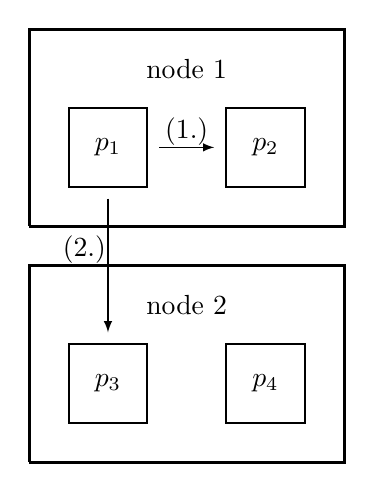
\begin{tikzpicture}
	
	
	\draw[main] (0,0) -- (4,0) -- (4,2.5)-- (0,2.5)-- (0,0);
	
	\node (rect) at (1,1) [draw,thick,minimum width=1cm,minimum height=1cm]  {$p_3$};
	\node (rect) at (3,1) [draw,thick,minimum width=1cm,minimum height=1cm]  {$p_4$};
	
	\draw[main] (0,3) -- (4,3) -- (4,5.5)-- (0,5.5)-- (0,3);
	
	\node (rect) at (1,4) [draw,thick,minimum width=1cm,minimum height=1cm]  {$p_1$};
	\node (rect) at (3,4) [draw,thick,minimum width=1cm,minimum height=1cm]  {$p_2$};
	
	\draw [arrow]  (1.5,4) to (2.5,4);
	\draw [arrow]  (1,3.5) to (1,1.5);
	
	\node at (2,5) {node 1};
	\node at (2,2) {node 2};
	
	\node at (2   , 4.2) {(1.)};
	\node at (0.7 , 2.7) {(2.)};
	
	
	\end{tikzpicture}
\end{minipage}%\hspace{0.5cm}
\begin{minipage}{0.5\textwidth}
	\vspace{-3cm}
	\begin{enumerate}
		\item \highlight{Copy} operation in memory
		\item \highlight{Sending} operation via network
	\end{enumerate}
\end{minipage}\hspace{0.5cm}

\end{frame}

%%%%%%%%%%%%%%%%%%%%%%%%%%%%%%%%%%%%%%%%%%%%%%%%%%%%%%%%%%%%%%%%%%%%%%%%%%%%%%%%
\begin{frame}{Hybrid implementation}
	\Large{\highlightB{MPI \& OpenMP}}
	\normalsize 

	\begin{minipage}{\textwidth}
		\centering
		\vspace{5mm}
		\begin{minipage}[t]{0.49\textwidth}
			MPI
			\begin{itemize}
				\item Process Based
				\item Communication on one node is copying
			\end{itemize}
		\end{minipage}
		\begin{minipage}[t]{0.49\textwidth}
			OpenMP
			\begin{itemize}
				\item Thread based
				\item shared memory
			\end{itemize}
		\end{minipage}
	\end{minipage}\\
	\Large{\vspace{5mm}\highlightB{Hybrid implementation}}\\
	\normalsize
	\vspace{5mm}
	\begin{itemize}
		\item MPI for communication between nodes and processors
		\item OpenMP parallelization on nodes
	\end{itemize}
\end{frame}

%%%%%%%%%%%%%%%%%%%%%%%%%%%%%%%%%%%%%%%%%%%%%%%%%%%%%%%%%%%%%%%%%%%%%%%%%%%%%%%%
\begin{frame}{Benchmarks}
	\Large{\highlightB{Hybrid implementation}}
	\normalsize random $10^7 \times 300 $ matrix
	
	\centering
	\scalebox{0.75}{
		% This file was created by matlab2tikz.
%
%The latest updates can be retrieved from
%  http://www.mathworks.com/matlabcentral/fileexchange/22022-matlab2tikz-matlab2tikz
%where you can also make suggestions and rate matlab2tikz.
%
\definecolor{mycolor1}{rgb}{0.00000,0.44700,0.74100}%
\definecolor{mycolor2}{rgb}{0.85000,0.32500,0.09800}%
\definecolor{mycolor3}{rgb}{0.92900,0.69400,0.12500}%
%
\begin{tikzpicture}

\begin{axis}[%
width=4.521in,
height=3.566in,
at={(0.758in,0.481in)},
scale only axis,
xmin=0,
xmax=82,
xlabel style={font=\color{white!15!black}},
xlabel={Number of Processors},
ymin=0,
ymax=9.2,
ylabel style={font=\color{white!15!black}},
ylabel={Speed up},
axis background/.style={fill=white},
axis x line*=bottom,
axis y line*=left,
legend style={at={(0.03,0.97)}, anchor=north west, legend cell align=left, align=left, draw=white!15!black}
]
\addplot [color=mycolor1, mark=x, mark options={solid, mycolor1}]
  table[row sep=crcr]{%
1	1\\
2	1.77735939387169\\
3	2.52863802350192\\
4	3.11057452110864\\
5	3.57893371259742\\
6	4.03232957353491\\
7	4.36130918935323\\
8	4.67456634083019\\
9	4.96249680943954\\
10	5.18947108447311\\
11	5.3335858729696\\
12	5.57220230405285\\
13	5.77127895622898\\
14	5.93399104352579\\
15	6.12791655430983\\
16	6.28131741232361\\
17	6.43572939044164\\
18	6.56942710425942\\
19	6.66259136120854\\
20	6.80310003314158\\
21	6.8629704671702\\
22	6.95050381730676\\
23	7.0026864165578\\
24	6.92879415004413\\
25	7.08846366609532\\
26	6.9958134809417\\
27	7.1537590661212\\
28	7.24624355476011\\
29	7.25119069143157\\
30	7.31806814919965\\
31	7.22171902050757\\
32	7.36785127600237\\
33	7.44764432815705\\
34	7.34539780745157\\
35	7.47319736513956\\
36	7.39081520555148\\
37	7.36910800431576\\
38	7.38777309107804\\
39	7.3566343535053\\
40	7.36808456825069\\
41	7.3834996696319\\
42	7.40378336312328\\
43	7.456569802935\\
44	7.05333438969816\\
45	7.43337465868924\\
46	7.50542861816718\\
47	7.43100346348961\\
48	7.42223143860942\\
49	7.52852347272102\\
50	7.53526729861858\\
51	7.46282625617122\\
52	7.5158741513344\\
53	7.43827655521545\\
54	7.33350964058771\\
55	7.52955433241322\\
56	7.39065330756398\\
57	7.4887936570745\\
58	7.45271351948498\\
59	7.52831060218862\\
60	7.4980138562886\\
61	7.55635737800393\\
62	7.50499860940941\\
63	7.29286168282935\\
64	7.37136455145628\\
65	7.63115952606785\\
66	7.64077429773524\\
67	7.56358721651871\\
68	7.52144777572109\\
69	7.62030948823592\\
70	7.56761881561985\\
71	7.54313696293749\\
72	7.54849495681635\\
73	7.64542909527055\\
74	7.52888257463664\\
75	7.49192020751487\\
76	7.61477515161743\\
77	7.57164503375542\\
78	7.23160517512624\\
79	7.56567980540322\\
80	7.43390429934376\\
};
\addlegendentry{EVP MPI}

\addplot [color=mycolor2, mark=o, mark options={solid, mycolor2}]
  table[row sep=crcr]{%
1	0.998599256860089\\
10	3.6920219080637\\
20	5.47626444971617\\
30	6.50911131728497\\
40	7.20530918150195\\
50	7.88185206239644\\
60	8.1636353091785\\
70	8.41029337130791\\
80	8.71579449228241\\
};
\addlegendentry{EVP hybrid}

\addplot [color=mycolor3, mark=+, mark options={solid, mycolor3}]
  table[row sep=crcr]{%
1	0.0644134706630309\\
2	0.121429810853809\\
3	0.203059284116331\\
4	0.256646008309173\\
5	0.311793484970624\\
6	0.364439924281973\\
7	0.393574070678828\\
8	0.443575708891036\\
9	0.462701461130375\\
10	0.506551521730153\\
11	0.512516891690243\\
12	0.541871584354609\\
13	0.551957233723199\\
14	0.600377954132289\\
15	0.576915306393257\\
16	0.609928612272296\\
17	0.633478092469771\\
18	0.639390998075112\\
19	0.632072161267883\\
20	0.653903688134457\\
21	0.703010508389928\\
22	0.727595190380761\\
23	0.751763534247655\\
24	0.805199339831863\\
25	0.815845004180602\\
26	0.86419572360972\\
27	0.894410122600335\\
28	0.908731664726426\\
29	0.925555040556199\\
30	0.939715730318634\\
31	0.954852378622423\\
32	1.01768985522706\\
33	1.02325037240064\\
34	1.11335064312017\\
35	1.08006937063289\\
36	1.14745102362626\\
37	1.15847348893686\\
38	1.19284917481663\\
39	1.22663164360764\\
40	1.16670591192576\\
41	1.22460234606197\\
42	1.23698676808494\\
43	1.27660035830304\\
44	1.34026449080253\\
45	1.29625770853619\\
46	1.39253918571556\\
47	1.38203854820538\\
48	1.40149434855347\\
49	1.40707510917746\\
50	1.44135858526514\\
51	1.48392878128024\\
52	1.53295285957849\\
53	1.53949413272853\\
54	1.49700663371601\\
55	1.56982074298877\\
56	1.57334435781624\\
57	1.54259173426033\\
58	1.71468049204225\\
59	1.66987981447088\\
60	1.63021852424936\\
61	1.68323557951482\\
62	1.6929761036298\\
63	1.68244403515131\\
64	1.73870543818423\\
65	1.8079538252603\\
66	1.88368433291433\\
67	1.78779788023682\\
68	1.90699247894872\\
69	1.83737322943827\\
70	1.94502520018575\\
71	1.91445438218831\\
72	1.94926845159181\\
73	1.96340438910897\\
74	1.90960707478878\\
75	1.97623336137365\\
76	1.99080609673254\\
77	1.97157999995408\\
78	1.92223091560331\\
79	1.91312355665274\\
80	1.94258302791729\\
};
\addlegendentry{SVD MPI}

\end{axis}
\end{tikzpicture}%
	}	
\end{frame}